\section{同伦映射诱导的同态}
\sourcepage{121}
现在研究重要的同伦概念。本节始终以 $I$ 表示闭单位区间 $[0,1]$。

\entry{定义}{2.7.1}设 $X,Y$ 为拓扑空间。若存在连续映射 $F:X\times I\to Y$，使对所有 $x\in X$ 有 $F(x,0)=h(x)$、$F(x,1)=k(x)$，则称连续映射 $h,k:X\to Y$ \textbf{同伦}，记为 $h\simeq k$。称 $F$ 为从 $h$ 到 $k$ 的\textbf{同伦}。\translatornote{原文首次写映射时用小写 $f$，随后均用 $F$；这里统一为 $F$。}

可以把 $F$ 看作一种方法，使 $t$ 从 $0$ 变到 $1$ 时，$h$ 连续地“变形”为 $k$。

我们将证明：若 $h,k:|K|\to|L|$ 同伦，则诱导的同调同态 $h_*,k_*$ 相同。这将导出重要结果：同调群是空间同伦型的不变量。

\entry{例}{2.7.2}设 $X=S^1$，则 $H_1(X)$ 为无限循环群。选取图 2.7.1 箭头表示的闭链 $z$ 为生成元。令 $T$ 为环面，$h,k:X\to T$ 如图所示。它们显然同伦，因为可以“把 $h$ 沿环推移”，直到与 $k$ 重合。几何上也清楚，闭链 $h_\#(z),k_\#(z)$ 同调。事实上，把环面右半部剖分为三角形并适当定向，得到 $2$ 维链 $d$，满足 $\partial d=h_\#(z)-k_\#(z)$。由于 $z$ 代表生成元，此时有 $h_*=k_*$。
\begin{center}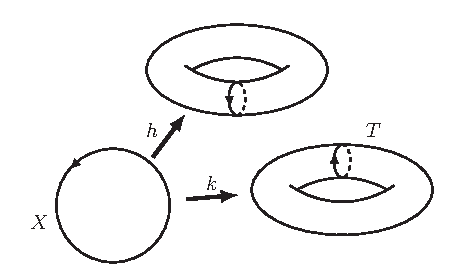
\includegraphics[width=82mm]{figures/2-7-1.pdf}\\图 2.7.1\end{center}
下面证明一般情形。需要两个预备结果。第一个是关于 $|K|\times I$ 的基本拓扑事实，将在下一节证明，见推论 2.8.7：\textit{乘积空间 $|K|\times I$ 的拓扑与子空间族 $\{\sigma\times I:\sigma\in K\}$ 相干。}第二个结果说明 $|K|\times I$ 是多面体。

\sourcepage{122--123}
\entry{引理}{2.7.3}若 $K$ 为复形，则 $|K|\times I$ 是某个复形 $M$ 的多胞体，且对每个 $\sigma\in K$，$\sigma\times I$ 为 $M$ 的某个子复形的多胞体，而 $\sigma\times0$、$\sigma\times1$ 都是 $M$ 的单形。

\noindent\textbf{证明：}对某个 $J$ 有 $|K|\subset E^J$，因而 $|K|\times I\subset E^J\times\R$。用定义重心剖分时的星形构造的一种变形，将它剖分为单形。

对 $p\geq0$，定义
\[
X_p=(|K|\times0)\cup(|K|\times1)\cup(|K^{(p)}|\times I).
\]
归纳剖分 $X_p$。$p=0$ 时，前两项是由各 $\sigma\times0$、$\sigma\times1$ 组成的复形的多胞体；第三项是由各边 $v\times I$ 及其顶点组成的复形的多胞体。它们的并为复形 $M_0$，底空间为 $X_0$。

一般地，假定 $M_{p-1}$ 的底空间为 $X_{p-1}$，并且当 $\dim s<p$ 时，$s\times I$ 为其子复形的多胞体。设 $\dim\sigma=p$，考察
\[
\begin{aligned}
\Bd(\sigma\times I)
&=(\sigma\times I)\setminus(\Int\sigma\times\Int I)\\
&=((\Bd\sigma)\times I)\cup(\sigma\times0)\cup(\sigma\times1).
\end{aligned}
\]
由于 $\Bd\sigma$ 为低维单形的并，这个边界为 $M_{p-1}$ 的子复形 $M_\sigma$ 的多胞体；边界紧致，所以 $M_\sigma$ 有限。令 $w_\sigma=(\widehat\sigma,1/2)$，锥 $w_\sigma*M_\sigma$ 的多胞体为 $\sigma\times I$。它与 $|M_{p-1}|$ 的交为两者某个共同子复形的多胞体。

令 $M_p$ 为 $M_{p-1}$ 与所有这些锥的并，最后令 $M=\bigcup_pM_p$。其底集恰为 $|K|\times I$，还须检验拓扑相同。

乘积拓扑与各 $\sigma\times I$ 相干，而 $|M|$ 的拓扑与其单形相干。若 $C$ 在乘积空间中闭，则 $C\cap(\sigma\times I)$ 在 $\sigma\times I$ 中闭。若 $M$ 的单形 $s$ 位于此乘积内，它是 $\sigma\times I$ 的子空间，因为二者紧致，均有从 $E^J\times\R$ 继承的拓扑。故 $C\cap s$ 在 $s$ 中闭，所以 $C$ 在 $|M|$ 中闭。

反过来，若 $C$ 在 $|M|$ 中闭，则每个 $C\cap s$ 在 $s$ 中闭。$\sigma\times I$ 是有限多个这样的单形的并，因此 $C\cap(\sigma\times I)$ 在 $\sigma\times I$ 中闭。由相干性，$C$ 在 $|K|\times I$ 中闭。\translatornote{原文最后一句误写为“因此 $\sigma$ 在 $|K|\times I$ 中闭”；论证所得应为 $C$ 闭。}\hfill$\square$

\entry{例}{2.7.4}若 $K$ 由一条边及其面组成，上述过程得到图 2.7.2 的剖分。若 $K$ 由一个 $2$ 维单形及其面组成，过程如图 2.7.3：左上为 $|K|\times I$，左下为剖分；右侧将各部分从 $(\widehat\sigma,1/2)$ 沿棱柱五个面的方向分离展示。
\begin{center}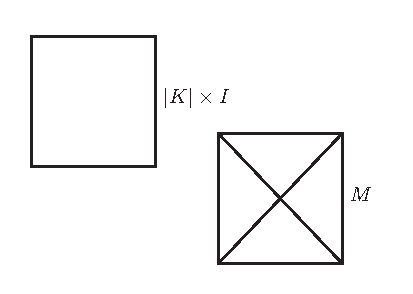
\includegraphics[width=74mm]{figures/2-7-2.pdf}\\图 2.7.2
\medskip

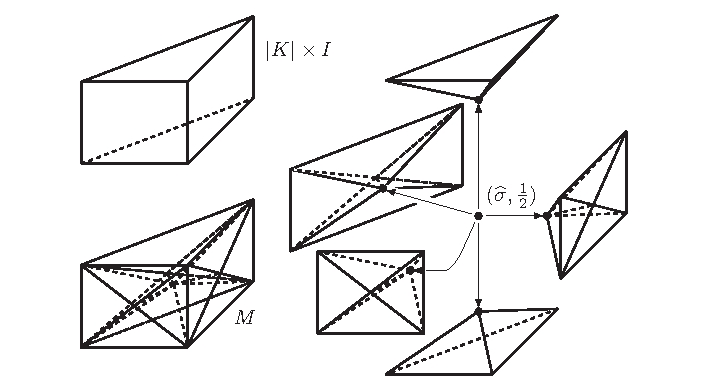
\includegraphics[width=122mm]{figures/2-7-3.pdf}\\图 2.7.3\end{center}

\sourcepage{124--125}
\entry{定理}{2.7.5}若映射 $h,k:|K|\to|L|$ 同伦，则 $h_*,k_*:H_p(K)\to H_p(L)$ 相等。约化同调也如此。

\noindent\textbf{证明：}取前一引理的复形 $M$，底空间为 $|K|\times I$，各 $\sigma\times0$、$\sigma\times1$ 为单形，各 $\sigma\times I$ 为子复形的多胞体。令 $F$ 为从 $h$ 到 $k$ 的同伦，定义 $i(x)=(x,0)$、$j(x)=(x,1)$。则 $i,j:K\to M$ 为单纯映射，且 $Fi=h$、$Fj=k$，见图 2.7.4。
\begin{center}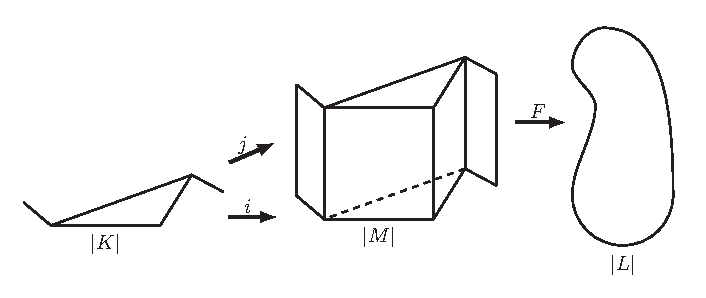
\includegraphics[width=122mm]{figures/2-7-4.pdf}\\图 2.7.4\end{center}
断言 $i_\#,j_\#$ 链同伦。对每个 $\sigma\in K$，令 $\Phi(\sigma)$ 为多胞体等于 $\sigma\times I$ 的子复形。它同胚于闭球，所以无环。面包含关系也保持，故 $\Phi$ 为无环载体，且同时承载 $i_\#,j_\#$。由定理 1.14.10，两链映射链同伦，因此 $i_*=j_*$。故
\[
h_*=F_*i_*=F_*j_*=k_*.
\]\hfill$\square$

结果直接推广到相对同调。若 $h,k:(|K|,|K_0|)\to(|L|,|L_0|)$ 之间存在同伦 $H$，且 $H$ 将 $|K_0|\times I$ 映入 $|L_0|$，则称两者\textbf{作为空间偶的映射同伦}。

\entry{定理}{2.7.6}若 $h,k$ 作为空间偶的映射同伦，则它们在相对同调上诱导相同同态。

\noindent\textbf{证明：}定理 2.7.5 的证明直接适用。$i,j$ 都将 $|K_0|$ 映入 $|K_0|\times I$，它们之间的链同伦也保持相应子复形。因此 $i_*=j_*$ 在相对同调中也成立，其余相同。\hfill$\square$

下面是由乘积拓扑的相干性得到的另一结果，后文将使用。

\entry{定理}{2.7.7}若 $f:K\to L$ 为连续映射 $h:|K|\to|L|$ 的单纯逼近，则 $f$ 同伦于 $h$。

\noindent\textbf{证明：}由引理 2.2.4，$f(x),h(x)$ 位于同一个单形内，所以直线同伦
\[
F(x,t)=(1-t)f(x)+th(x)
\]
将 $|K|\times I$ 映入 $|L|$。若 $L$ 有限，它作为到欧氏空间的映射连续，而 $|L|$ 具有子空间拓扑，所以 $F$ 连续。一般情形只需验证每个 $\sigma\times I$ 上的限制连续。

对 $x\in\sigma$，令 $\tau_x$ 为内部包含 $h(x)$ 的单形。因为 $h(\sigma)$ 紧致，各 $\tau_x$ 只有有限多个，令它们及其面组成 $L_\sigma$。由引理 2.2.4，$f(x)\in\tau_x$，故 $F$ 将 $\{x\}\times I$ 映入 $\tau_x$，于是将 $\sigma\times I$ 映入 $|L_\sigma|$。$L_\sigma$ 有限，其底空间有欧氏子空间拓扑，故此限制连续。再复合连续包含 $|L_\sigma|\to|L|$，得到所需连续性。\hfill$\square$

我们知道同胚空间有同构的同调群。事实上，一种较弱的关系也能保证这一点，即同伦等价。

\entry{定义}{2.7.8}若存在映射 $f:X\to Y$、$g:Y\to X$，使 $gf\simeq i_X$、$fg\simeq i_Y$，则称 $X,Y$ \textbf{同伦等价}（homotopy equivalent），或\textbf{具有相同同伦型}（homotopy type）。$f,g$ 称为\textbf{同伦等价映射}，$g$ 称为 $f$ 的\textbf{同伦逆}。

此关系的对称性、自反性显然，传递性留作习题。因此同伦等价是等价关系。

若 $X$ 与单点空间具有相同同伦型，则称 $X$ \textbf{可缩}（contractible）。这等价于 $i_X$ 同伦于常值映射。例如，单位球可缩，因为 $F(x,t)=(1-t)x$ 是恒等映射到常值映射的同伦。

\sourcepage{126--127}
\entry{定理}{2.7.9}若 $f:|K|\to|L|$ 为同伦等价，则 $f_*$ 为同构。特别地，若 $|K|$ 可缩，则 $K$ 无环。

\noindent\textbf{证明：}若 $g$ 为同伦逆，则 $g_*$ 为 $f_*$ 的逆。\hfill$\square$

一般的同伦等价难以直观描绘，但有一类在几何上较易理解。

\entry{定义}{2.7.10}从 $X$ 到 $A$ 的\textbf{形变收缩}（deformation retraction）是连续映射 $F:X\times I\to X$，满足
\[
\begin{aligned}
F(x,0)&=x&& (x\in X),\\
F(x,1)&\in A&& (x\in X),\\
F(a,t)&=a&& (a\in A,\ t\in I).
\end{aligned}
\]
若存在这样的 $F$，则称 $A$ 为 $X$ 的\textbf{形变收缩核}（deformation retract）。

令 $r(x)=F(x,1)$，则 $r:X\to A$ 为收缩映射。设 $j:A\to X$ 为包含映射，则 $rj=i_A$；而 $F$ 是 $i_X$ 与 $jr$ 之间的同伦，且整个过程中 $A$ 的每一点保持不动。因此 $r,j$ 互为同伦逆。

可以把形变收缩看作逐渐将 $X$ 坍缩到子空间 $A$，同时固定 $A$ 的每一点。这类同伦等价能够几何地描绘。直观上，若 $A$ 为 $X$ 的形变收缩核，$B$ 为 $A$ 的形变收缩核，则 $B$ 为 $X$ 的形变收缩核；这也容易证明。

\entry{定理}{2.7.11}单位球面 $S^{n-1}$ 是去心欧氏空间 $\R^n\setminus\{0\}$ 的形变收缩核。

\noindent\textbf{证明：}令 $X=\R^n\setminus\{0\}$，定义
\[
F(x,t)=(1-t)x+t\frac{x}{\|x\|}.
\]
它将从原点出发的每条开射线收缩到与单位球面的交点，满足要求。\hfill$\square$

\entry{推论}{2.7.12}若 $n\ne m$，则 $\R^n$ 与 $\R^m$ 不同胚。

\noindent\textbf{证明：}若有同胚 $h$，限制后得到 $\R^n\setminus\{0\}$ 与 $\R^m\setminus\{p\}$ 的同胚，其中 $p=h(0)$。后者又同胚于 $\R^m\setminus\{0\}$。由定理，$S^{n-1}$ 与 $S^{m-1}$ 同伦等价。但当 $n\ne m$ 时，前者的 $n-1$ 维约化同调为 $\Z$，后者为零，矛盾。\hfill$\square$

\entry{例}{2.7.13}两个圆周的楔和与字母 $\theta$ 具有相同同伦型。设 $X$ 为图 2.7.5 的平面双孔椭圆区域。左侧箭头说明如何将其坍缩为两个圆周的楔和，右侧说明如何坍缩为 $\theta$。两空间都与 $X$ 同伦等价，因而彼此同伦等价。
\begin{center}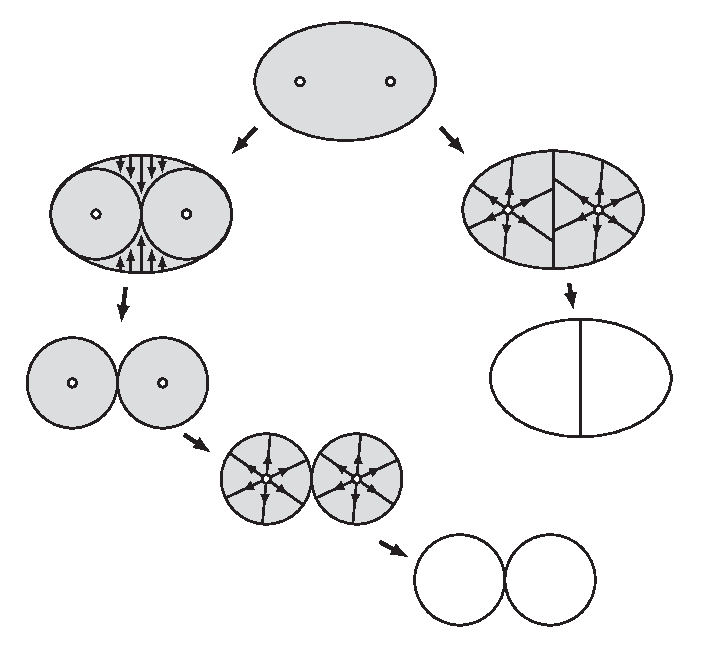
\includegraphics[width=122mm]{figures/2-7-5.pdf}\\图 2.7.5\end{center}

\sourcepage{128--129}
这一情形比乍看更一般。一个有趣事实是，每个同伦等价都能用形变收缩表述。具体地，$X,Y$ 同伦等价，当且仅当存在空间 $Z$ 及嵌入 $h:X\to Z$、$k:Y\to Z$，使 $h(X),k(Y)$ 都是 $Z$ 的形变收缩核，见 [Whi78]、[Fuc71]。\translatornote{本段前后讨论形变收缩，而原文此处写作 homotopy retracts；这里按其所述标准结果译为形变收缩核。}此事实有助于直观理解同伦等价的几何含义。

同伦等价是计算同调群的有力工具。给定复形 $K$，证明其底空间同伦等价于同调已知的空间，通常比直接计算其同调容易。下面的习题说明这一想法。

\subsection*{习题}
\begin{enumerate}
\item 证明同伦等价是任意空间族上的等价关系。
\item 证明：若 $A$ 为 $X$ 的形变收缩核，$B$ 为 $A$ 的形变收缩核，则 $B$ 为 $X$ 的形变收缩核。
\item 将下列空间按同伦等价分类。假定它们都是复形的多胞体，计算各自同调群。
\begin{enumerate}[label=(\alph*)]
\item Möbius 带。
\item 环面。
\item 实心环面 $B^1\times S^1$。\translatornote{原文写 $B^1\times S^1$，但通常实心环面为 $B^2\times S^1$；前者是环带。此处保留原式。}
\item 去掉一点的环面。
\item 去掉两点的环面。
\item 去掉一点的 Klein 瓶。
\item 去掉 $z$ 轴的 $\R^3$。
\item 去掉圆周 $\{x^2+y^2=1,z=0\}$ 的 $\R^3$。
\item (g)、(h) 两空间的交。
\item 从 $S^3$ 中去掉两个相链的圆周。
\item 从 $S^3$ 中去掉两个不相链的圆周。
\end{enumerate}
\item 证明：若 $\dim K=n$，则 $|K|$ 的覆盖维数至少为 $n$。
\item 不使用 $|K|\times I$ 是复形底空间这一事实，按下列步骤证明定理 2.7.5：
\begin{enumerate}[label=(\alph*)]
\item 设 $K,L$ 有限，$h:|K|\to|L|$。证明存在 $\epsilon>0$，使只要 $k$ 对每个 $x$ 满足 $|h(x)-k(x)|<\epsilon$，就有 $h_*=k_*$。［提示：选择 $K'$，使 $h(\overline{\operatorname{St}(v,K')})\subset\operatorname{St}(w,L)$。$\epsilon$ 足够小时，把 $h$ 换为 $k$ 仍成立。］
\item 证明 $K,L$ 有限时的定理。
\item 证明一般情形。［提示：每条闭链都由有限子复形承载。］
\end{enumerate}
\end{enumerate}
